\documentclass[12pt,a4paper]{report}
\usepackage[utf8]{inputenc}
\usepackage{amsmath}
\usepackage{amsfonts}
\usepackage{amssymb}
\usepackage{graphicx}
\usepackage{float}
\input defs.tex
\bibliographystyle{alpha}
\graphicspath{ {./figures/} }

\title{Game Theoretic Solutions to Power Control in MIMO Communications Systems}
\author{Peter Hartig}

\begin{document}
\maketitle

%\begin{abstract}
%This work investigate resource allocation strategies for such systems and in particular, those strategies minimizing system overhead. 
%\end{abstract}
%
%\newpage
\tableofcontents
\newpage

\chapter{Introduction}
\section{Introduction}
Modern communication systems often incorporate numerous, uncoordinated users competing for a limited resource.
In this work, a game theoretic approach considers a wireless communications network with uncoordinated  macrocell and femtocell users. The goal of this approach is to find Nash Equilibrium in which Femtocell base stations optimize their utility while ensuring macrocell users intercept interference below a given threshold. 
Previous work has shown solutions for systems in which the femtocell base stations transmit over a SISO channel; thus the MIMO case is investigated here. 
One of the primary goals of this work is to achieve Nash Equilibrium via distributed solutions which minimize system overhead. As seen in the following, the most general setup of this game does not permit such solutions and therefore a refined problem is purposed.


\section{Relevant Tools/Theory}

It is useful to first review relevant tools for solving such games. Together, these tools provide a series of steps to reach Nash Equilibrium via a distributed solutions. 

\begin{enumerate}
\item The Concave N-Person game a framework for proving existence and uniqueness of NE for games fulfilling certain criteria.

\begin{itemize}
\item
\textbf{Definition:} A game in which the individual player optimization problems are concave and the strategy set resulting from problem constraints (potentially player coupled) is convex.
\item 
\textbf{Existence of Nash Equilibrium:} Pure Strategy NE exist for Concave N-Person  games \cite[Thm1]{rosen1964existence}. 
\item
\textbf{Uniqueness of Nash Equilibrium:} To prove uniqueness of NE for Concave N-Person  games, the "Normalized Nash Equilibrium" is introduced.
First a weighted sum of the player utility functions is taken.
\begin{equation}
\sigma(u,r)  = \Sigma_{\mathrm{f=1}}^{\mathrm{F}} r_{\mathrm{f}}U_{\mathrm{f}}(), \; 
r_{\mathrm{f}} \geq 0
\end{equation}
 The function $G(b,r) $ is defined as the Jacobian of $g(b,r) $ which is defined as
\begin{enumerate}
\item  
\begin{equation}
g(b,r)= 
\begin{bmatrix}
r_1 \nabla U_{1}(b)
\\
r_2 \nabla U_{2}(b)
\\
\vdots\\
r_F \nabla U_{F}(b)
\end{bmatrix}
\end{equation}

\begin{itemize}
\item
Negative Definiteness of the matrix $[G(b,r)+G^{T}(b,r)] $ is a sufficient condition for Diagonally Strict Concavity of $\sigma(u,r)$ which is a sufficient condition for uniqueness of a NNE \cite[Thm4]{rosen1964existence}

\end{itemize}

\end{enumerate}
\end{itemize}
\item The Potential function of a game.
\begin{itemize}
\item
\textbf{Definition:} A function
$ \Psi()$ which satisfies:
\begin{equation}\label{potential_game_condition}
\frac{\partial \Psi(x)}{\partial u_{f,i}}
 =
 \frac{\partial U_(x)}{\partial u_{f,i}}
\end{equation}
\item Global optima to the Potential function correspond to NE of the game.
\item If a Concave N-Person game game admits a potential function, the potential function will be concave. NE may then be found efficiently by convex optimization tools. 
\end{itemize}



\item Distributed Optimization
\begin{itemize}
\item Distributed solutions minimize the system overhead required in sharing
\begin{itemize}
\item Begin with a central optimization problem.
\item For the dual of the central problem
\item Evaluate if problem can be separated into sub-problems each with independent optimization variables.
\item Perform an ascent of the dual problem by iterating between solving for the dual function of the sub-problems and then broadcasting these solutions to perform the gradient step of the dual problem. 

\end{itemize} information between network users. 
\end{itemize}
\item Concave Programming?

\end{enumerate}
\subsection{Using the tools}
(May want to make a flow chart?)
The typical usage of these tools is:
first verify existence and uniqueness for a Normalized NE of the game using n-concave games,
second find a centralized version n-concave game which will be a concave function over a concave set,
find a distributed solution to the single convex problem resulting from the potential funciton.


\section{Outline}
Look at how the tools described above will be used in the work. 
\begin{itemize}
\item 
\ref{genmodel} Introduces the system model for the most general setup of the problem.
\item 
\ref{genproblem} Introduces various tools for solving for Nash Equilibrium and analyzes the general setup for compatibility with these tools. 
\item
\ref{conmodel} Provides refinements to the system model in order to allow for ...
\item 
\ref{conproblem} Details solving the full problem ...
\item 
details numerical comparisons of the two proposed methods for identifying Nash Equilibrium of the game. 
\end{itemize}
\chapter{System Model}

\section{General System Model}\label{genmodel}

\subsection{Players: Femtocell Base Stations}


Each player of the game, a Femtocell base station $f \in \{1 ... F\}$ (FC-BS), is characterized by:
\begin{itemize}
\item 
$T_f$ antennas with which to transmit to $K_f$ femtocell users (it is assumed that $T_f \geq K_f$).
\\
\item 
	Precoding matrix $\mathbf{U}_{\mathrm{f}} \in \mathbb{C}_{T_f \times K_f}$ such that the transmitted 		
	signal is $\mathbf{s}_{\mathrm{f}
	}= \mathbf{U_{\mathrm{f}}}\mathbf{x_{\mathrm{f}}}$. Here $\mathbf{x_{\mathrm{f}}}$ is the 		
	vector of symbols for users of FC-BS $f$ normalized such that $E[\|\mathbf{x}_{\mathrm{f,i}}
	\|_2^2]=1$ and $E[\mathbf{x}_{\mathrm{f}}\mathbf{x}_{\mathrm{f}}^H]=\mathbf{I}$.
\\
\item 
	Power constraint $trace(\mathbf{U}_f^H\mathbf{U}_f) \leq P^{Total}_{f} $.

\item 
	Cost function $U_f() =
	\sum_{\mathrm{i=1}}^{\mathrm{K_f}}
    	 U_{\mathrm{f,i}}(\gamma_{\mathrm{f,i}}) $
    	in which all $U_{\mathrm{f,i}}()$ are non-decreasing in argument. (No assumption about concavity is made at this point)

\item 
	Knowledge of the downlink channel matrix $\mathbf{H_\mathrm{f}} \in \mathbb{C}_{K_f \times T_f} $ to the $K_f$ users.
% TODO(Simulate degradation with incomplete CSI solution?)
\\
\item
	 FC-BSs are assumed to be spaced far apart in distance such that FC-BS $f$ 
	 causes no interference to the users of any other FC-BS. As a result, $U_f()$ is indepenent of all other FC-BSs.
\end{itemize}

\subsection{Macrocell Users}
Macrocell users $m \in \{1 ... M\}$ introduce constraints into the game. These users are characterized by:

\begin{itemize}
\item 
	Received interference constraint
	$\sum^F_{f=1} \mathbf{\tilde{h}}_{\mathrm{m,f}}^T  \mathbf{U_{\mathrm{f}}} 						
	\mathbf{U_{\mathrm{f}}^{\mathrm{H}}} \mathbf{\tilde{h}_{\mathrm{m,f}}^*} \leq I^{Threshold}		
	_{\mathrm{m}} $.

\item 
	FC-BS $f$ is assumed to know the downlink channel matrix $\tilde{\mathbf{H}_{\mathrm{f}}} \in \mathbb{C}_{M \times T_f}$ to all $M$ Macrocells users.
\\
\end{itemize}

\subsection{Femtocell Users}
\begin{itemize}

\item User $i$ of FC-BS $f$ has signal to interference plus noise ratio (SINR):
	\begin{equation*}
	\gamma_{\mathrm{f,i}} = \frac{\|\mathbf{h^H_{\mathrm{f,i}}u_{\mathrm{f,i}}}\|^2}
	{\sigma^2_{noise}   +
	\underbrace{
	 \sum_{\mathrm{\tilde{f}}=1,\mathrm{\tilde{f}}\neq f}^{\mathrm{F}} \sum_{\mathrm{u=1}}^{K_{\mathrm{\tilde{f}}}}
	\|\mathbf{h^H_{\mathrm{\tilde{f},u}}u_{\mathrm{\tilde{f},i}}}\|^2}_{\mathrm{inter-cell}}
	 + 
	 \underbrace{
	 \sum_{\mathrm{\tilde{k}\neq i}}^{\mathrm{K_f}}
	 \|\mathbf{h^H_{\mathrm{f,\tilde{k}}}u_{\mathrm{f,\tilde{k}}}}\|^2}_{\mathrm{intra-cell}}}
	  \; \mathrm{i \in \{1 ... K_f\}}\end{equation*}
\\
with AWGN $\sim \mathcal{CN}(0,\sigma^2_n)$
\\

Assuming negligible inter-cell interference, this reduces to
	\begin{equation*}
	\gamma_{\mathrm{f,i}} = \frac{\|\mathbf{h^H_{\mathrm{f,i}}u_{\mathrm{f,i}}}\|^2}
	{\sigma^2_{noise} 
	 + \sum_{\mathrm{\tilde{k}\neq i}}^{\mathrm{K_f}}
	  \|\mathbf{h^H_{\mathrm{f,\tilde{k}}}u_{\mathrm{f,\tilde{k}}}}\|^2}
	  \; \mathrm{i \in \{1 ... K_f\}}
	\end{equation*}
\\


\end{itemize}





\subsection{General Optimization Problem}

Each player $f$ attempts to maximize utility function $U_f()$ while satisfying the interference constraints imposed by the macro cell users and a transmission power constraint. 
\par




	\begin{subequations}
	\label{optim}
	\begin{align}
	    \underset{\mathbf{U}_{\mathrm{f}} }{\text{argmin}} \;
	    & - \sum_{\mathrm{i=1}}^{\mathrm{K_f}}
    	U_{\mathrm{f,i}}(\gamma_{\mathrm{f,i}}) \label{player_opt} \\
	    \text{subject to} \; &
	   \sum^F_{f=1} \mathbf{\tilde{h}}_{\mathrm{m,f}}^T  \mathbf{U_{\mathrm{f}}}		
	\mathbf{U_{\mathrm{f}}^{\mathrm{H}}} \mathbf{\tilde{h}_{\mathrm{m,f}}^*} \leq I^{Threshold}		
	_{\mathrm{m}} & m \in \{1 ...M\} 
		\label{interference_const_gen}\\
        & trace(\mathbf{U_f^H}\mathbf{U_f}) \leq P^{Total}_{f} \label{power_const_gen}\\
        & \langle \mathbf{h_{f,j}}\mathbf{u_{f,i}} \rangle =0\ & \; \forall j \in \{1... K_f\}\backslash i ,\; \forall i \in \{1 ... K_f\} \label{zf_const_gen}
	\end{align}
	\end{subequations}
	
In order to ensure the resulting game admits a potential function, $\mathbf{U}_{\mathrm{f}}$ is restricted to the set of zero-forcing matrices by constraint \eqref{zf_const_gen}.	
	
\subsection{Concave N-Person game analysis of general setup}
The convexity of the resulting problem is analyzed in order to fulfill the conditions of a Concave N-Person game. 

\begin{enumerate}


\item
The constraints form a convex, closed and bounded set. 

\begin{itemize}

\item
	Constaint \eqref{interference_const_gen} contains $M$ quadratic constraints on $\mathbf{U_f}$ and 
	can be rewritten as 

\begin{gather*}
	\sum_{f=1}^F
	trace(\mathbf{U_f^H} \mathbf{\tilde{h}_{m,f}} \mathbf{\tilde{h}_{m,f}^H} \mathbf{U_f} )\leq 
	I^{Threshold}_{m}.
\end{gather*}
This can be further decomposed into  
	\begin{gather*}
	\sum_{f=1}^F
	\sum_{i=1}^{f_i}
	\mathbf{u_{\mathrm{f,i}}^H}\mathbf{\tilde{h}_{\mathrm{m,f}}} \mathbf{\tilde{h}}_{\mathrm{m,f}}^H
	\mathbf{u_{\mathrm{f,i}}} \leq I^{Threshold}_{m}
	\end{gather*}
in which the term $ \mathbf{\tilde{h}_{\mathrm{m,f}}} \mathbf{\tilde{h}}_{\mathrm{m,f}}^H$ is  a positive semi-definite matrix and is, therefore, a convex set 
\cite[p.8,9]{BoV:04}. 
%This is essentially high dimensional ellipsoid.


\item \
	Constraint \eqref{power_const_gen} can be similarly decomposed into the sum
	\begin{gather*}
		\sum_{i=1}^{K_f}\mathbf{u_{\mathrm{f,i}}^{\mathrm{H}}} \mathbf{I} 		
		\mathbf{u_{\mathrm{f,i}}} \leq  P^{Total}_{f}
	\end{gather*}
	in which $\mathbf{I}$ is positive definite and 			
	therefore the constraint is strictly convex for the same 		
	reason as \eqref{interference_const_gen}.

\item 
	Constaint \eqref{zf_const_gen} is an affine constraint. 
		\begin{gather*}
		\langle \mathbf{h_{\mathrm{f,j}}}\mathbf{u_{\mathrm{f,i}}} \rangle =0
		\end{gather*}
%Note that affine constaints to not have to satisfy Slater's condition
\end{itemize}


\item Concavity of the utility function
\begin{itemize}
\item 
Due to constraint \eqref{zf_const_gen}, $\gamma_{\mathrm{f,i}}$ takes the form
	\begin{equation}\label{zf_snr}
	\gamma_{\mathrm{f,i}} = \frac{\|\mathbf{h^H_{\mathrm{f,i}}u_{\mathrm{f,i}}}\|^2}
	{\sigma^2_{noise}  
	}
	= 
	\frac{\mathbf{u^H_{\mathrm{f,i}}h_{\mathrm{f,i}}h^H_{\mathrm{f,i}}u_{\mathrm{f,i}}}}
	{\sigma^2_{noise}  
	}
	\end{equation}
	As $\mathbf{h}_{\mathrm{f,i}}\mathbf{h}^H_{\mathrm{f,i}}$ is positive semi-definite, $\gamma_{\mathrm{f,i}}$ is convex in ${\mathbf{u}_{\mathrm{f,i}}}$. 
\item
The composition $U_{\mathrm{f,i}}(\gamma_{\mathrm{f,i}}) $ is concave only if $U_{\mathrm{f,i}}() $ is concave and non-increasing; violating the non-decreasing definition of $U_{\mathrm{f,i}}() $.
If $U_{\mathrm{f,i}}() $ is a general non-decreasing function, the resulting
 function to \emph{maximize} is quasiconvex \cite[p.~102]{BoV:04}. In the case
  that $U_{\mathrm{f,i}}() $ is  non-decreasing and convex, the resulting
   function to \emph{maximize} is convex and therefore, concave programming can
    potentially be used to find an optima. 
\end{itemize}

\end{enumerate}

\subsection{Potential Game for General Problem}
Under the current system model, the game is not a Concave N-Person game. Nevertheless, the game may still admit a potential function whose global optima will correspond to a Normalized Nash Equilibrium.


\section{Concave System Model}\label{conmodel}

The general setup of this game seen in the previous section prohibits the use of tools to identify NE efficiently in this context. 
The following adaption of the general problem permits a unique Nash Equilibrium to be found via a single convex problem which may be distributed across players of the game.

\subsection{Players: Femtocell Base Stations}
Femtocells are adapted from the general setup by the following:
\begin{itemize}
\item 
	FC-BSs with multiple antennas ($T_f \geq 1$) can beamform their transmission using the precoding 	
	matrix $\mathbf{U}_{\mathrm{f}} \in \mathbb{C}_{T_f \times K_f}$ .
	The columns of $\mathbf{U}_{\mathrm{f}}$ are normalized such that 
	 $\|\mathbf{u}_{\mathrm{fi}}\|^2 =1 \;\forall i \in \{1 ... K_f\}$.
\\

\item 
$\mathbf{U}_f$ is selected as an inverse to $\mathbf{H_\mathrm{f}}$.
Such that
\begin{gather*}
\langle \mathbf{h_{f,j}}\mathbf{u_{f,i}} \rangle =0\  \; \forall j \in \{1... K_f\}\backslash i ,\; \forall i \in \{1 ... K_f\}
\end{gather*}

\item  
	FC-BS $f$ allocates  transmission power using the diagonal, power allocation  	
	matrix $\mathrm{diag}(\mathbf{p}_{\mathrm{f}})$ with $p_{\mathrm{fi}} \geq 0, \forall i \in \{1 ... K_f\}$
such that the transmitted 		
	signal is 
	$\mathbf{s}_{\mathrm{f}	}= \mathbf{U_{\mathrm{f}}} 
	\mathrm{diag}(\mathbf{p}_{\mathrm{f}})^{\frac{1}{2}}
	\mathbf{x_{\mathrm{f}}}$.
\\
\item 
	FC-BS $f$ has power constraint:
	\begin{gather*}
	trace(E[\mathbf{s}_\mathrm{f}\mathbf{s}_\mathrm{f}^H]) =
	\sum_{\mathrm{i=1}}^{\mathrm{K_{\mathrm{f}}}} p_{\mathrm{fi}}
	  \leq P^{Total}_{f} 
	  	\end{gather*}

% TODO(Simulate degradation with incomplete CSI solution?)


\item 
	Cost function $U_f() =
	\sum_{\mathrm{i=1}}^{\mathrm{K_f}}
    	U_{\mathrm{f,i}}(\gamma_{\mathrm{f,i}}) $
    	in which all $U_{\mathrm{f,i}}()$ are non-decreasing and \emph{concave} in argument.

\end{itemize}

\subsection{Macro Cell Users}
Same as the general setup.

\subsection{Femtocell Users}
Same as the general setup.

\subsection{Optimization Problem of player $f$}


	\begin{subequations}
	\label{optim}
	\begin{align}
	    \underset{\mathbf{p}_{\mathrm{f}} }{\text{minimize}} \;
	    & - \sum_{\mathrm{i=1}}^{\mathrm{K_f}}
    	U_{\mathrm{f,i}}(p_{\mathrm{f,i}}) \label{player_opt_c} \\
	    \text{subject to} \; &
	  \sum^F_{f=1} \mathbf{\tilde{h}}_{\mathrm{m,f}}^T  \mathbf{s}_{\mathrm{f}} 						
	\mathbf{s_{\mathrm{f}}^{\mathrm{H}}} \mathbf{\tilde{h}_{\mathrm{m,f}}^*} 
	=
	\sum_{\mathrm{f=1}}^{\mathrm{F}}	\sum_{\mathrm{i=1}}^{\mathrm{K_f}}
	p_{\mathrm{fi}}\|\tilde{h}_{\mathrm{mf}}^T u_{\mathrm{fi}}\|^2_2
	\leq I^{Threshold}		
	_{\mathrm{m}} & m \in \{1 ...M\} 
		\label{interference_const_c}\\
        & trace(\mathbf{s}_\mathrm{f}\mathbf{s}_\mathrm{f}^H) =
        	\sum_{\mathrm{i=1}}^{\mathrm{K_{\mathrm{f}}}} p_{\mathrm{fi}}
	   \leq P^{Total}_{f}  \label{power_const_c}\\
        & p_{\mathrm{f,i}} \geq 0 &  i \in \{1 ...K_{\mathrm{f}}\} \label{pos_power_const_c}
	\end{align}
	\end{subequations}

Note that because $U_{\mathrm{f}}$ is pre-selected as an inverse to  $\mathbf{H_\mathrm{f}}$, constraint \eqref{zf_const_gen} has been removed.
\subsection{Concave N-Person game analysis of concave setup}

Sufficient conditions for a concave problem are:

\begin{enumerate}

\item
The constraints form a convex, closed and bounded set. 

\begin{itemize}

\item
	Constaint \eqref{interference_const_c} contains $M$ affine constraints on $diag(\mathbf{p_{\mathrm{f}}})$.

\begin{gather*}
	  \sum^F_{f=1} \mathbf{\tilde{h}}_{\mathrm{m,f}}^T  \mathbf{s}_{\mathrm{f}} 						
	\mathbf{s_{\mathrm{f}}^{\mathrm{H}}} \mathbf{\tilde{h}_{\mathrm{m,f}}^*} 
	=
	\sum_{\mathrm{f=1}}^{\mathrm{F}}	\sum_{\mathrm{i=1}}^{\mathrm{K_f}}
	p_{\mathrm{fi}}\|\tilde{h}_{\mathrm{mf}}^T u_{\mathrm{fi}}\|
	\leq I^{Threshold}_{\mathrm{m}} 
\end{gather*}

\item \
	Constraint \eqref{power_const_c} is  afine in $diag(\mathbf{p_{\mathrm{f}}})$.
	
\item \
	Constraint \eqref{pos_power_const_c} is affine in $diag(\mathbf{p_{\mathrm{f}}})$.
\end{itemize}

%Note that affine constaints to not have to satisfy Slater's condition

\item The utility function is assumed concave in its argument $p_{\mathrm{f,i}}$.

\end{enumerate}

This problem satisfies the conditions for the Concave N-Persion game and therefore a pure strategy Nash Equilibrium exists due to 
\cite[Thm1]{rosen1964existence}.

Next, the conditions for unqiueness of this NE are verified. As the utility function $U_{\mathrm{fi}}(p_{\mathrm{fi}})$ is (strictly?) concave, (differentiable?), and independent of all $p_{\mathrm{fj}}$ the matrix $[G(b,r)+G^{T}(b,r)] $ will be diagonal with values on the diagonal $<0$. As $[G(b,r)+G^{T}(b,r)] $ is negative definite the Normalized Nash Equilibrium are unique \cite[Thm4]{rosen1964existence}.

\subsection{Potential Game for Concave Problem}

\textbf{Potential Function:} The proposed potential function satisfying \eqref{potential_game_condition} is 

\begin{gather*} \label{Potential_Function}
\Psi(\mathbf{p}) = \sum_{f = 1}^{F} U_f(\mathbf{p_{\mathrm{f}}}) 
\end{gather*}

resulting in the single optimization problem in which $\mathbf{p}= [\mathbf{p_{\mathrm{1}}},\mathbf{p_{\mathrm{2}}}...\mathbf{p_{\mathrm{F}}}]$
	
		\begin{subequations}
	\label{optim}
	\begin{align}
	    \underset{\mathbf{p}}{\text{minimize}}
	    & \; \Psi(\mathbf{p}) \label{potential_game} \\
	    \text{subject to} \; &
	  \sum^F_{f=1} \mathbf{\tilde{h}}_{\mathrm{m,f}}^T  \mathbf{s}_{\mathrm{f}} 						
	\mathbf{s_{\mathrm{f}}^{\mathrm{H}}} \mathbf{\tilde{h}_{\mathrm{m,f}}^*} \leq I^{Threshold}		
	_{\mathrm{m}} & m \in \{1 ...M\} 
		\label{interference_const}\\
        & trace(\mathbf{s}_\mathrm{f}\mathbf{s}_\mathrm{f}^H)  \leq P^{Total}_{f}  \label{power_const}
        & \forall f \in \{1 ... F\}\\
        & p_{\mathrm{f,i}} \geq 0 &  \forall i \in \{1 ...K_{\mathrm{f}}\} \; \forall f \in \{1 ... F\}\label{pos_power_const}
	\end{align}
	\end{subequations}

%\begin{theorem}\label{distributed}
%\cite{ghosh2015normalized}
%If a game's potential function is strictly concave and the derivative of the function with respect to the individual players variables are independent of the other player variables, then there exists a distributed solution.
%\end{theorem}

\subsection{Distributed Solution to the Game}
A distribtued solution to \eqref{potential_game} is now proposed  minimize communication overhead between processes in the optimization (in this case players and macro users).
\subsubsection{Central Problem Resulting from Potential Game}
As distributed implementation of dual ascent \cite[p.~8,9]{boyd2011distributed} is proposed to solve the potential game. 
\\
\begin{multline}
L(\mathbf{U,\lambda}) = 
\;
\sum_{f=1}^F U_f() 
+
\sum_{\mathrm{m=1}}^M \lambda_{\mathrm{m}}
(	  \sum^F_{f=1} \mathbf{\tilde{h}}_{\mathrm{m,f}}^T  \mathbf{s}_{\mathrm{f}} 						
	\mathbf{s_{\mathrm{f}}^{\mathrm{H}}} \mathbf{\tilde{h}_{\mathrm{m,f}}^*} - I^{Threshold}		
	_{\mathrm{m}} )
\\
+ 
\sum_{f=1}^F
\chi_{\mathrm{f}}(trace(\mathbf{s}_\mathrm{f}\mathbf{s}_\mathrm{f}^H)-P^{Total}_{f} )
+
\sum_{f=1}^F 
\sum_{i=1}^{K_f}
\nu_{\mathrm{f,i}}(-p_{\mathrm{f,i}})
\end{multline}

The corresponding dual function and dual problem are then 
\begin{gather*}
g(\lambda,\nu) = \underset{\mathbf{U}}{\mathrm{argmin}}\;L(\mathbf{U,\lambda})
\end{gather*}
\begin{gather*}
g(\lambda,\nu) = \underset{\lambda}{\mathrm{argmax}}\;\underset{\mathbf{U}}{\mathrm{argmin}}\;L(\mathbf{U,\lambda})
\end{gather*}
.



This dual function can be decomposed into $F$ component functions
\begin{multline}
g_f(\lambda,\nu) = \underset{\mathbf{p_f}}{\mathrm{argmin}}
\{
\;
U_f() 
+
\sum_{\mathrm{m=1}}^M \lambda_{\mathrm{m}}
(\mathbf{\tilde{h}}_{\mathrm{m,f}}^T  \mathbf{s}_{\mathrm{f}} 						
	\mathbf{s_{\mathrm{f}}^{\mathrm{H}}} \mathbf{\tilde{h}_{\mathrm{m,f}}^*} - \frac{I^{Threshold}_{\mathrm{m}}}{F})
\\
+ 
\chi_{\mathrm{f}}(trace(\mathbf{s}_\mathrm{f}\mathbf{s}_\mathrm{f}^H)-P^{Total}_{f} )
+
\sum_{i=1}^{K_f}
\nu_{\mathrm{f,i}}(-p_{\mathrm{f,i}})\}
\end{multline}
\\

The following algorithm achieves reach the NE of the potential game. 
\subsubsection{Distributed Algorithm 1}\label{algo1}

\begin{enumerate}
\item 
Individual players (FC-BSs) can solve $ g_f(\lambda,\nu) $ independently.
\begin{itemize}
\item Setting $\frac{\partial g_f(\lambda,\nu)}{\partial p_{\mathrm{f,i}}} = 0$ 

\item 
Solving for $p_{\mathrm{fi}}$ using \eqref{zf_snr} yields

\begin{gather}
p_{\mathrm{fi}} = (\sum_{\mathrm{m=1}}^{\mathrm{M}}\lambda_{\mathrm{m}}\|\mathbf{\tilde{h}}_{m,f}^T \mathbf{U_f}_{\mathrm{i}}\|^2_2
+\chi_{f} \|\mathbf{u}_{\mathrm{f,i}}\|^2_2
-\nu_{\mathrm{f,i}}
 )^{-1}
  - \sigma^2_n
\end{gather}

\end{itemize}
\item 
Using $g(\lambda,\nu) = \sum_{f=1}^{F}g_f(\lambda,\nu)$ and the calculus of subgradients $\partial g(\lambda,\nu) = \sum_{f=1}^{F} \partial g_f(\lambda,\nu)$, the dual variables can updated using:

\begin{gather}
\lambda_{\mathrm{m}}^{\mathrm{k+1}} = (
\lambda_{\mathrm{m}}^{\mathrm{k}}
+
\alpha^{\mathrm{k}}*
(
\underbrace{
\sum _{\mathrm{f=1}}^{\mathrm{F}}
\sum _{\mathrm{i=1}}^{\mathrm{K_{\mathrm{f}}}}
p_{\mathrm{fi}}
\|\mathbf{\tilde{h}}_{\mathrm{mf}}^T \mathbf{u_{\mathrm{fi}}}\|^2_2}_{Interference}
- I_{\mathrm{m}}
))^+
\end{gather}
performed at the macro cell users,

\begin{gather}
\chi_{\mathrm{f}}^{\mathrm{k+1}} = (
\chi_{\mathrm{f}}^{\mathrm{k}}
+
\alpha^{\mathrm{k}}*
(\underbrace{\sum_{\mathrm{i=1}}^{\mathrm{K_{\mathrm{f}}}} p_{\mathrm{fi}}}_{Used Power} - P_{\mathrm{f}}^{Total}) )^+
\end{gather}
performed at individual FC-BSs, and 

\begin{gather}
\nu_{\mathrm{fi}}^{\mathrm{k+1}} = (
\nu_{\mathrm{fi}}^{\mathrm{k}}
+
\alpha^{\mathrm{k}}*
(-p_{\mathrm{fi}}))^+
\end{gather}
also performed at individual FC-BSs.
As each of dual variable in this update is an inequality constraint, the implementation of this algorithm directly enforces non-negativity using 
$(arg)^+$.
Step size $\alpha^{\mathrm{k}}$ is predefined and constant.
 % must satisfy  $\sum_{\mathrm{k=1}}^{\infty} \alpha^{\mathrm{k}}$ (cite).



\end{enumerate} 
Notice that these updates only require the information detailed in the problem description. 

\chapter{Simulation and Results}
\subsection{Simulation System Description}
The Heterogeneous Network is simulated by randomly placing $F $ and M Macro Cell Users within a predefined area. Each FC-BS is assigned $K_{\mathrm{f}}$ unique Femto Users. All channels between FC-BS and users (both Femtro and Macro) are simulated using rayleigh fading and attenuation coefficient $d^{- \beta}$ with $\beta =2$ and $d$ as the distance between user and base-station.
FC-BS $f$ initializes power to user $i$ as $p_{\mathrm{fi}} = \frac{P^{P_{\mathrm{f}}^{Total}}}{K_{\mathrm{f}}} $ such that the corresponding power constraint is not violated. 
Dual variables are intitialized 
\begin{figure}[h!]
	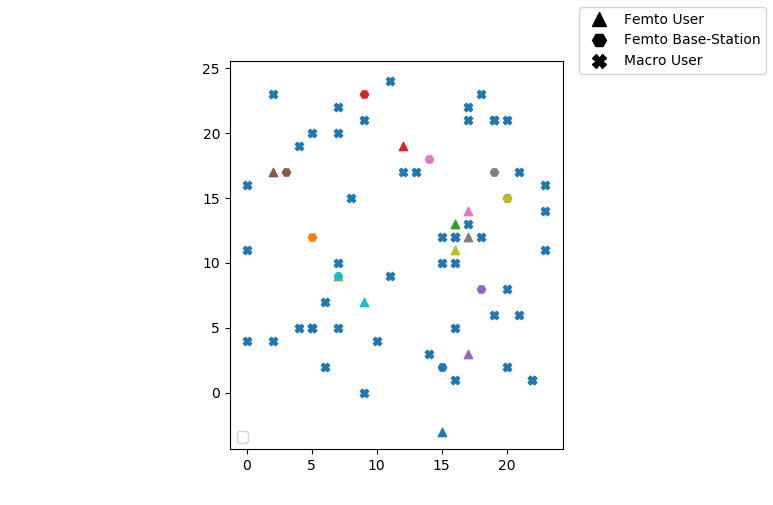
\includegraphics[width=\textwidth,height = 10cm]{figures/system_figure}
	  \caption{Simluation Setup}
\end{figure}

\subsection{Simulation Results}
Using the algorithm in \ref{algo1} convergence to a Nash Equilibrium is observed over a variety of scenarios to observe the convergence towards a NE in the network. 
\subsubsection{Simulation Results for Concave Setup}
Figure \ref{fig:power} depicts convergence to Nash Equilibrium for different 
transmission power constraints. When users are given sufficient power to violate the interference constraints of the macro users, the convergence is slowed and less stable.
\begin{figure}[h!]
	  \caption{Increasing FC-BS Power}
	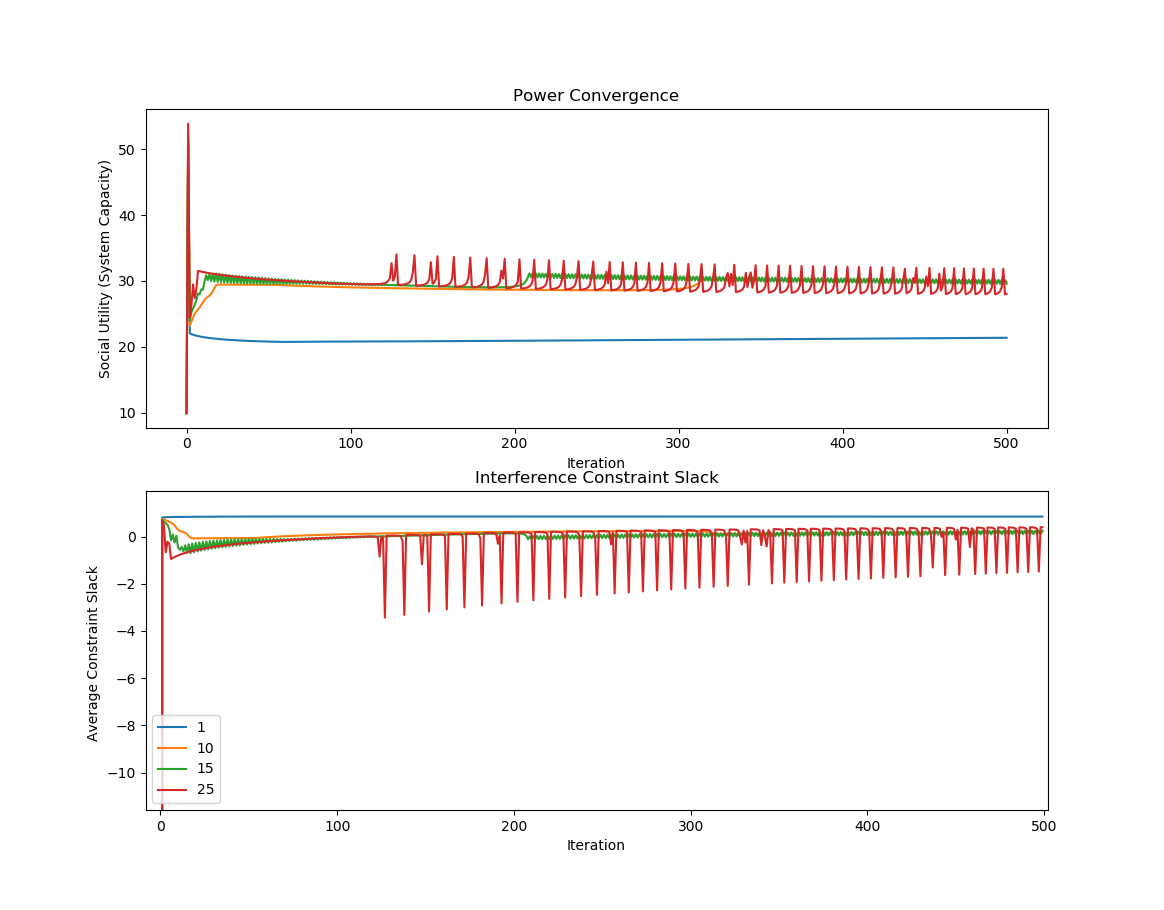
\includegraphics[width=\textwidth,height = 7cm]{figures/power_active}
	  \label{fig:power}
\end{figure}

Figure \ref{fig:inc_fc} depicts convergence to Nash Equilibrium for different FC-BS densities in the network. As the number of FC-BS is increase in a constant area with constant Macro Users, the average FC-BS utility decreases. 
 
\begin{figure}[H]
	  \caption{Increasing FC-BS Density}
	  	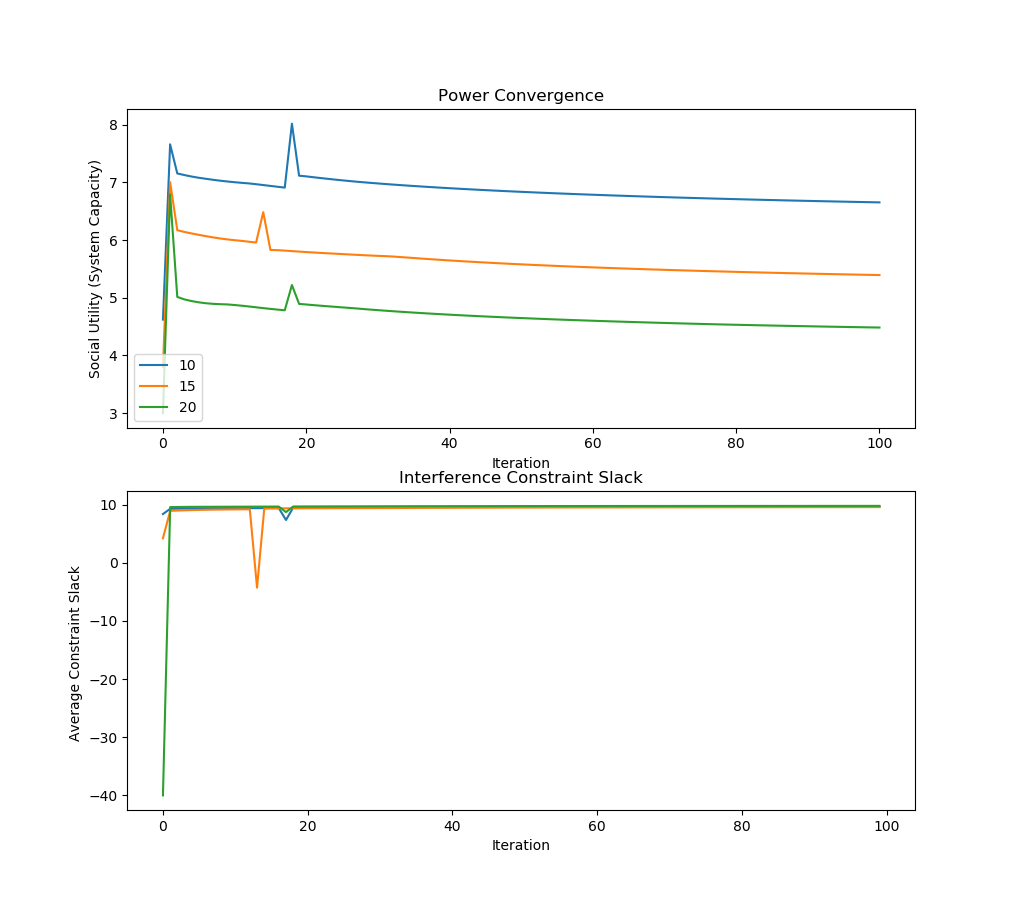
\includegraphics[width=\textwidth,height = 7cm]{figures/increasing_fcbs}
	  \label{fig:inc_fc}
\end{figure}


Figure \ref{fig:dec_tol} depicts convergence to Nash Equilibrium for decreasing interference tolerance of the Macro Cell Users in the network. 

\begin{figure}[H]
	  \caption{Decreasing Interference Tolerance }
	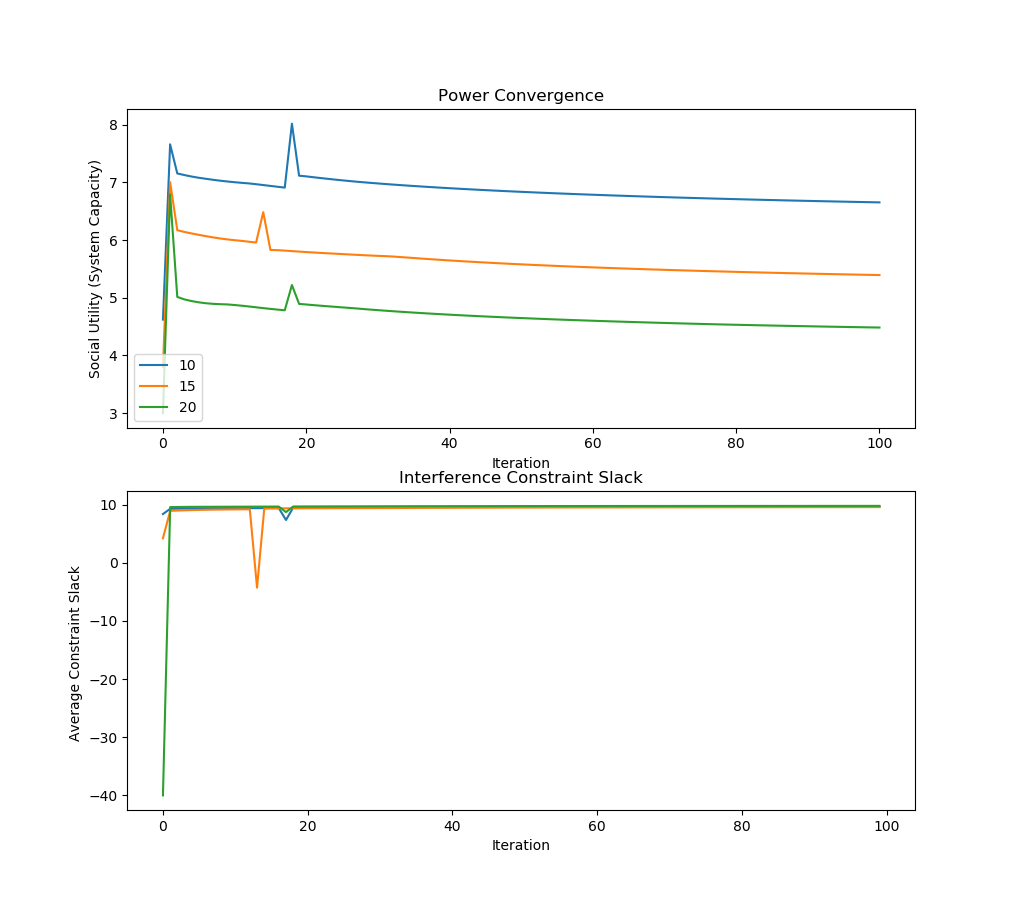
\includegraphics[width=\textwidth,height = 7cm]{figures/increasing_fcbs}
		  \label{fig:dec_tol}
\end{figure}

Figure \ref{fig:beamformers} depicts convergence to Nash Equilibrium for different Zero-Forcing beamformers chosen according to (Explanation). 

Compare different beamformer choices and their convergence
\begin{figure}[H]
	  \caption{Base Station Beamformer Comparison}
	  	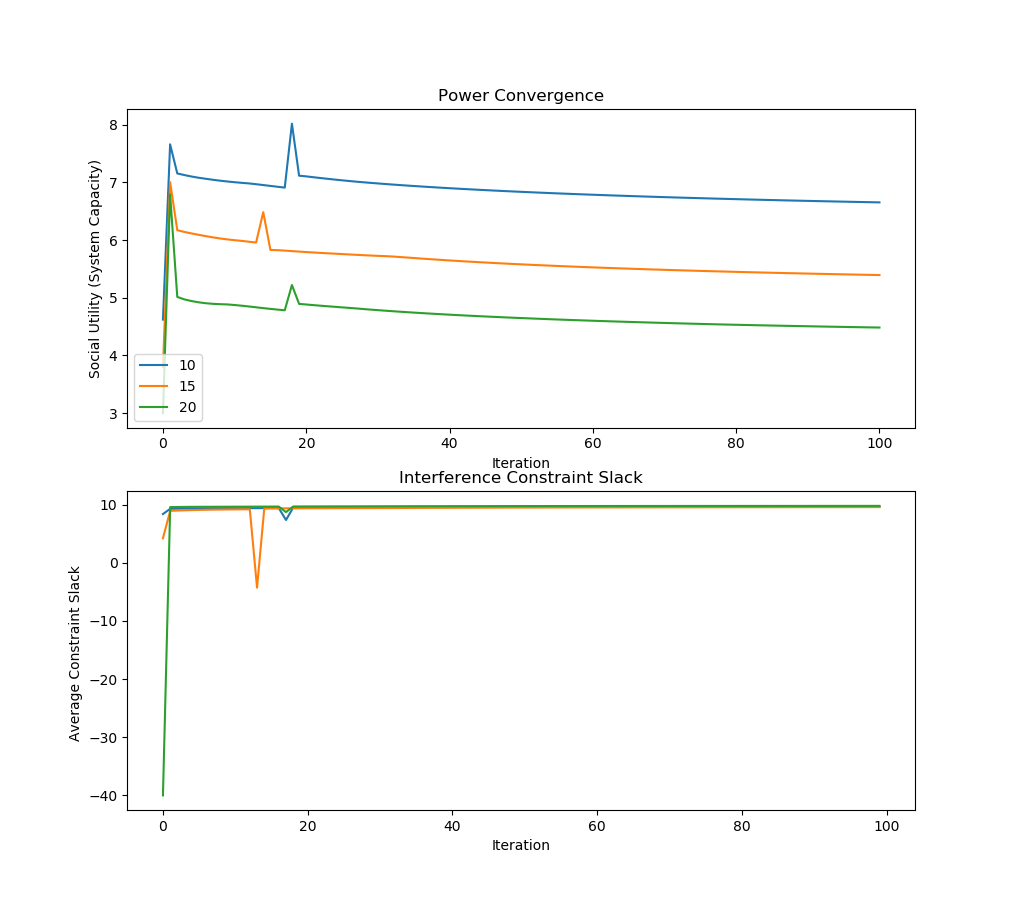
\includegraphics[width=\textwidth,height = 7cm]{figures/increasing_fcbs}
	  \label{fig:beamformers}
\end{figure}

\chapter{Conclusion}

\newpage
\bibliography{gt_report}
\end{document}
